\documentclass[11pt,a4paper]{article}

\usepackage[margin=1in]{geometry}
\usepackage{amsmath,amssymb}
\usepackage{graphicx}
\usepackage[hidelinks]{hyperref}
\usepackage{booktabs}
\usepackage{caption}
\usepackage{microtype}
\usepackage[numbers,sort&compress]{natbib}

\captionsetup{font=small,labelfont=bf}
\setlength{\parskip}{0.05em}
\setlength{\parindent}{1.3em}

\title{\vspace{-2.5em}\textbf{Autoimmune Cloud: when automated remediation\\
becomes the outage}}
\author{Aniket Pradeep Kulkarni \quad\textbullet\quad Yang Yang\\[0.2em]
\small CITS4403 Computational Modelling, The University of Western Australia}
\date{\vspace{-0.8em}\small October 2026}

\begin{document}
\maketitle
\vspace{-1.5em}

\begin{abstract}
\noindent
Cloud platforms detect faults statistically and remove suspect service instances
without human review. Because a removed instance sheds its traffic onto its
neighbours, and elevated traffic is what an anomaly detector is built to notice,
the remediation system is itself a cascade process running on the infrastructure
it protects. We model this as a cellular automaton in which cells carry load,
fail when overloaded, and are separately removed when telemetry crosses a
detector threshold. Two thresholds follow analytically from the local rule and
are confirmed by simulation: a critical spare capacity $\alpha_c = 1/|N|$ and a
critical sensitivity $\theta_c = (1 + 1/|N|)/(1+\alpha)$, the second notable for
omitting detector accuracy entirely. A platform with twice the headroom needed
to absorb one failure is destroyed by its own remediation system, total damage
is U-shaped in sensitivity, and a third result states when a safe threshold
exists at all. Both the U-shape and the topology results prove conditional on
how a failing cell's load is shared among its neighbours---a modelling choice
usually left implicit, which we therefore measure under two explicit rules.
\end{abstract}

\vspace{-0.5em}
\section{Background and research aims}

A cloud platform of any scale runs far more service instances than operators can
watch, so anomaly detection over telemetry is commonly wired directly to
remediation: an instance whose metrics look wrong is drained, killed and
replaced with no human in the loop. Every detector then faces an unavoidable
trade-off, because the telemetry of a faulty instance and of a merely busy one
overlap, so any threshold trades false positives against false negatives. That
is a property of overlapping distributions, not a defect of a classifier, and is
normally treated as a tuning problem.

That framing assumes the two costs are independent, which is wrong once
response is automated. In a monitored system a false positive costs an
engineer's attention, and ten cost ten times one. In an automated system it
\emph{removes a healthy instance}, whose traffic lands on its neighbours---and
elevated utilisation is exactly the signature the detector was trained to flag,
so those neighbours become candidates for removal in turn. False positives
compound rather than add. The parallel is autoimmunity: past some point a more
aggressive response destroys more healthy tissue than it saves.

Our research question is: \emph{how do detector sensitivity, spare capacity and
neighbourhood structure jointly determine total system damage in an automated
remediation system?} We test three hypotheses. \textbf{H1}: damage is U-shaped
in sensitivity, with an interior minimum set by spare capacity and connectivity
rather than detector accuracy. \textbf{H2}: beyond some critical sensitivity
the remediation system alone is supercritical, destroying a platform on which no
physical cascade could propagate. \textbf{H3}: a heterogeneous dependency-graph
neighbourhood changes the character of the transition.

\section{Related work and contribution}

The load-redistribution half of the model belongs to a well-established family:
the Bak--Tang--Wiesenfeld sandpile \citep{bak1987} and the Drossel--Schwabl
forest-fire automaton \citep{drossel1992} spread a local excess to lattice
neighbours and exhibit self-organised criticality, the Motter--Lai model
\citep{motter2002} applies this to networks, and the robust-yet-fragile
character of scale-free networks under targeted attack \citep{albert2000} is
standard there.

Our model departs from these in three ways. First, removal is permanent within
an episode rather than conservative: sandpile toppling redistributes grains and
the cell recovers, so load diffuses, whereas here a failed cell is gone and load
\emph{concentrates} on a shrinking set of survivors. Second, and centrally,
there is a \emph{second removal mechanism driven by the state the first one
creates}. No existing cascade automaton contains a detector; our quarantine rule
reads the utilisation that redistribution produces and removes cells because of
it, closing a positive feedback loop that load redistribution alone does not
possess. This is the contribution. Third, we decompose damage by cause and
derive the critical sensitivity analytically rather than only measuring it.

The model is not one of the examples excluded by the brief. The sandpile and the
graph models appear in the unit textbook \citep{downey2018}; we reuse the
lattice-spreading idea and the \texttt{networkx} generators, and re-implement
the method of \citet{clauset2009} from the paper. No code was copied from
open-source projects. The detector-coupled quarantine rule, the two-route state
design, the damage decomposition, the analytic results and the topology
comparison are original.

\section{Model specification}

The platform is a $W \times H$ lattice of cells, each one service instance, with
states drawn from $\{\textsc{healthy}, \textsc{degraded}, \textsc{shedding},
\textsc{down}, \textsc{quarantining}, \textsc{quarantined}\}$. Neighbourhoods
are von Neumann (4) or Moore (8), identical for every cell, with fixed
non-periodic boundaries, and the update is synchronous. Each cell carries a
real-valued load $\ell_i$, as the sandpile carries a grain count, moving only
between neighbours so the rule stays strictly local; capacity is
$c_i = (1+\alpha)\,\ell_i(0)$. Every lattice is initialised with all cells
\textsc{healthy} and unit load, $\ell_i(0) = 1$, so $\alpha$ is literally the
fraction of headroom each cell holds and damage is read directly in cells.

The transition rule has two phases. A cell first gathers load shed by neighbours
that failed on the previous step,
\begin{equation}
\ell_i(t{+}1) = \ell_i(t) + \!\!\sum_{j \in N(i),\, s_j \in \{\textsc{shed},\,\textsc{quar}\}}\!\! \frac{\ell_j}{r_j},
\label{eq:gather}
\end{equation}
and then transitions. \textsc{shedding} becomes \textsc{down} and
\textsc{quarantining} becomes \textsc{quarantined}, both with load set to zero;
\textsc{down} and \textsc{quarantined} are absorbing. A \textsc{healthy} cell
becomes \textsc{degraded} with probability $p$ per step, representing a genuine
fault such as a bad deployment or a memory leak. A serving cell becomes
\textsc{shedding} if $\ell_i(t{+}1) > c_i$, and otherwise becomes
\textsc{quarantining} if its telemetry exceeds the threshold $\theta$.

\textsc{shedding} and \textsc{quarantining} are one-step transient states,
playing the role \textsc{burning} plays in the forest-fire automaton: they let a
failed cell hand its load to its neighbours using only local information.
Keeping \textsc{down} and \textsc{quarantined} distinct lets damage be
attributed to overload as against remediation.

The divisor $r_j$ in Equation~\ref{eq:gather} is a choice cascade models usually
leave implicit, and it matters enough to measure both ways. Under the
\emph{shared} rule $r_j = |N(j)|$, load divides among all static neighbours and
whatever reaches an already-removed cell is recorded as dropped; under the
\emph{live-only} rule $r_j$ counts only serving neighbours, so nothing is lost
but survivors absorb more. The first models a load balancer with a stale view of
membership, the second a perfect view, and they give materially different
answers.

Telemetry is
\begin{equation}
\mathrm{tel}_i = \frac{\ell_i}{c_i} + \delta\,\mathbb{1}[s_i = \textsc{degraded}] + \varepsilon_i, \qquad \varepsilon_i \sim \mathcal{N}(0,\sigma^2),
\end{equation}
utilisation plus an offset if the cell is faulty plus noise. The noise makes the
faulty and busy populations overlap, which is the reason the problem exists.
Characterising the detector by $\delta$ and $\sigma$ rather than training a
classifier makes its \emph{quality} and \emph{operating point} independently
variable.

Principal assumptions: capacity is scalar, requests homogeneous, redistribution
completes within one timestep, cells are binary, removal is permanent within an
episode, and faults are independent. Section~\ref{sec:disc} states what each
bounds.

\section{Analytic predictions}

Two thresholds follow directly from the rule and serve as validation gates
rather than results. A failing cell spills $\ell/|N|$ to each neighbour, so a
neighbour rises to $\ell(1 + 1/|N|)$ and the cascade halts exactly when that
still fits within capacity:
\begin{equation}
\alpha_c = \frac{1}{|N|}.
\end{equation}
A von Neumann lattice thus needs 25\% headroom to absorb one failure and a Moore
lattice only 12.5\%, the load spreading across twice as many cells.

The detector supplies a second removal route with its own critical point. A cell
that has absorbed one dead neighbour reads $(1 + 1/|N|)/(1+\alpha)$; if $\theta$
lies below that, every such cell is flagged, and quarantining it floods its own
neighbours in turn, so that
\begin{equation}
\theta_c = \frac{1 + 1/|N|}{1+\alpha}.
\label{eq:thetac}
\end{equation}
What Equation~\ref{eq:thetac} omits matters as much as what it contains: the
safe operating point is fixed by spare capacity and by how load redistributes,
and \emph{no term for detector accuracy appears}. A platform may improve its
detector and remain equally close to the cliff.

\section{Experimental protocol}

Two protocols are used, both with fixed, logged seeds. \emph{Single-cascade
trials} seed one failure at the centre with no fault process and measure both
thresholds. \emph{Episodes} run under a background fault rate with no seeded
failure, so every loss originates either from the fault process or from
remediation itself; these give the damage decomposition, reported as cell-steps
spent degraded and undetected, cells lost to overload, and healthy cells removed
by the detector, each normalised by lattice size. Table~\ref{tab:params} lists
the standing values and the ranges swept.

\begin{table}[t]
\centering\scriptsize
\caption{Standing parameters and swept ranges; values not being swept take the
value shown. Loads and damage are in cells, $\theta$, $\delta$ and $\sigma$ in
units of utilisation. Lattices are $50\times50$ (episodes), $60\times60$ (cascade
figure) and $41\times41$ (gate sweeps), with $8$ replicate seeds per $\theta$ and
$12$ on the fine sweep; graphs use $N = 900$ at mean degree $4$ with $300$
single-cell failures per topology, $800$ for the degree analysis.}
\label{tab:params}
\begin{tabular}{@{}llll@{}}
\toprule
\textbf{Symbol} & \textbf{Meaning} & \textbf{Value} & \textbf{Swept over} \\
\midrule
$\ell_i(0)$ & initial load per cell & $1$ (uniform) & --- \\
$\alpha$    & spare capacity        & $0.6$ & $0.05$--$1.0$ \\
$|N|$       & neighbourhood size    & $4$ (von Neumann) & $4$, $8$ (Moore) \\
$\theta$    & detector threshold    & --- & $0.70$--$1.20$ \\
$\delta$    & fault signal          & $0.35$ & $0.06$--$0.60$ \\
$\sigma$    & telemetry noise (s.d.) & $0.03$ & $0.01$--$0.05$ \\
$p$         & fault rate per cell-step & $2\times10^{-4}$ & --- \\
$T$         & observation horizon   & $150$ steps & --- \\
\bottomrule
\end{tabular}
\end{table}

These choices are deliberate rather than fitted. $\alpha = 0.6$ sits well above
$\alpha_c = 0.25$, so such a platform cannot cascade physically and any loss is
attributable to remediation; $\delta = 0.35$ and $\sigma = 0.03$ place the
detector inside the separable regime of Equation~\ref{eq:sep}, so a safe
threshold exists and the question is whether it is found; and $p$ is small
enough that faults arrive singly rather than in overlapping waves.

Four protocol choices follow an audit that found the earlier treatment unsound;
two changed published numbers. A run under ongoing noise has no fixed point, so
stochastic runs execute a stated horizon rather than stopping at the first quiet
step; faults and telemetry noise are drawn from separate streams indexed by
timestep and cell, so a seed fixes the potential inputs and the detector setting
alone varies; load addressed to an already-removed cell is recorded as dropped,
so every episode balances; and degree-ordered selections break ties by ascending
index. Appendix~\ref{app:protocol} gives the verification evidence for each.

\begin{sloppypar}
Every number below comes from \path{experiments/report_numbers.py} via
\path{data/report_numbers.json}, from which the figures are also drawn, so text
and plots cannot drift apart.
\end{sloppypar}

\section{Results}
\label{sec:results}

\paragraph{Both analytic gates hold.}
Measured thresholds match Equations (3) and (4) to within sweep resolution
(Figure~\ref{fig:gates}): $\alpha_c$ is recovered exactly at $0.2500$ and
$0.1250$, and the eight $\theta_c$ measurements deviate by at most $0.002$ from
prediction.

\begin{figure}[t]
\centering
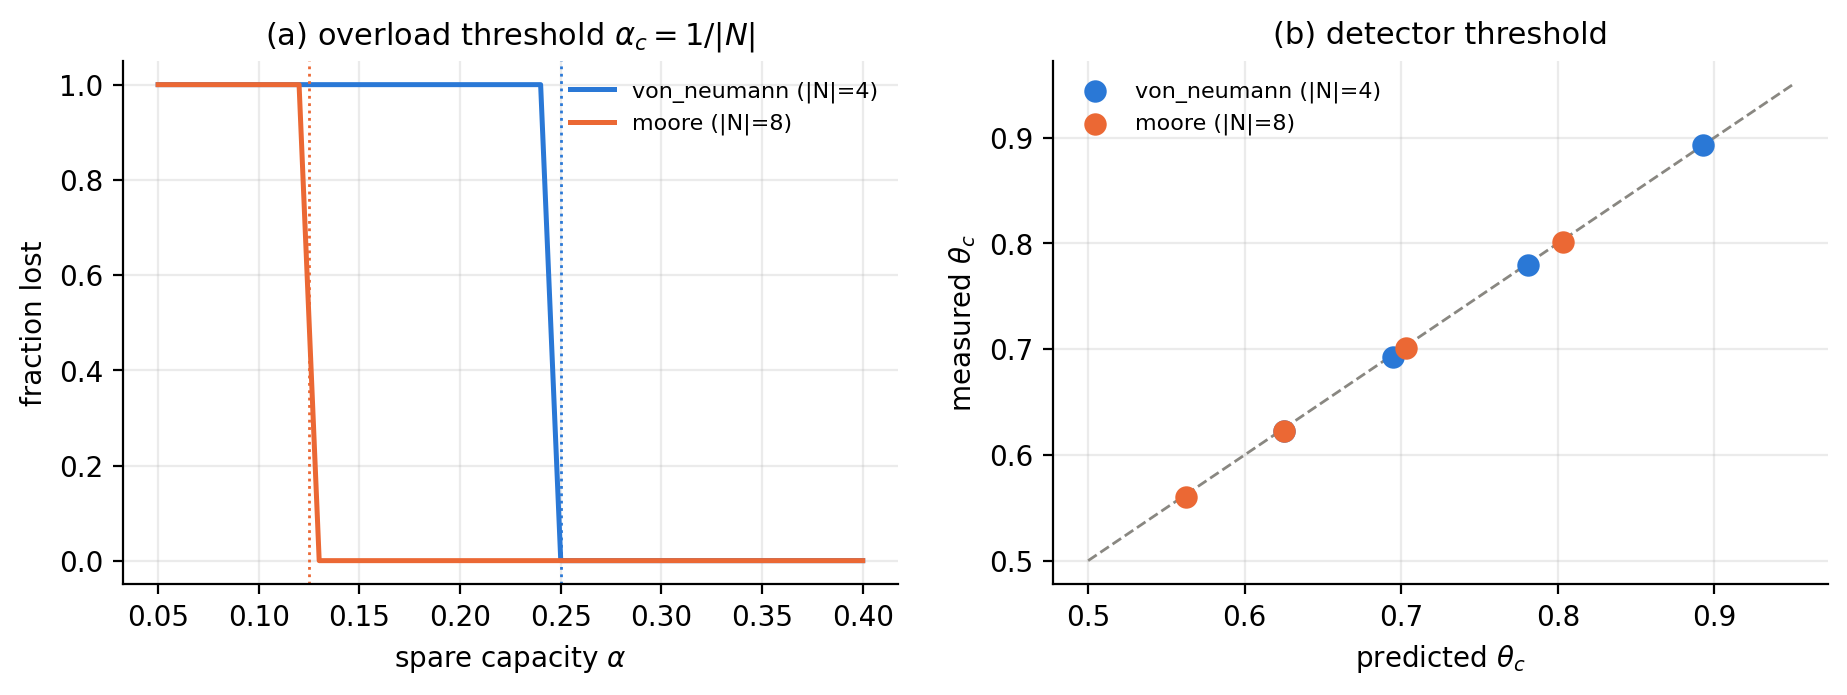
\includegraphics[width=\textwidth]{figures/fig2_gates.png}
\caption{Validation. (a) Fraction of the lattice lost against spare capacity;
dotted lines mark the predicted $\alpha_c = 1/|N|$. (b) Measured against
predicted critical detector threshold across two neighbourhoods and four
capacity levels; the dashed line is $y=x$.}
\label{fig:gates}
\end{figure}

\paragraph{Remediation alone destroys a subcritical platform (H2).}
At $\alpha = 0.6$ a seeded failure with the detector disabled removes exactly one
cell and nothing follows: a physical cascade cannot propagate. Enabling the
detector at $\theta = 0.82$ or below destroys the entire lattice over the
150-step horizon
(Figure~\ref{fig:cascade}); at $\theta = 0.85$ and above, nothing happens. Every
loss is self-inflicted. Most cells are recorded as lost to overload rather than
to the detector---at $\theta = 0.80$, 3322 against 278---but they overloaded only
because the detector had already removed their neighbours, so the detector is
the cause even where it is not the proximate mechanism.

\begin{figure}[t]
\centering
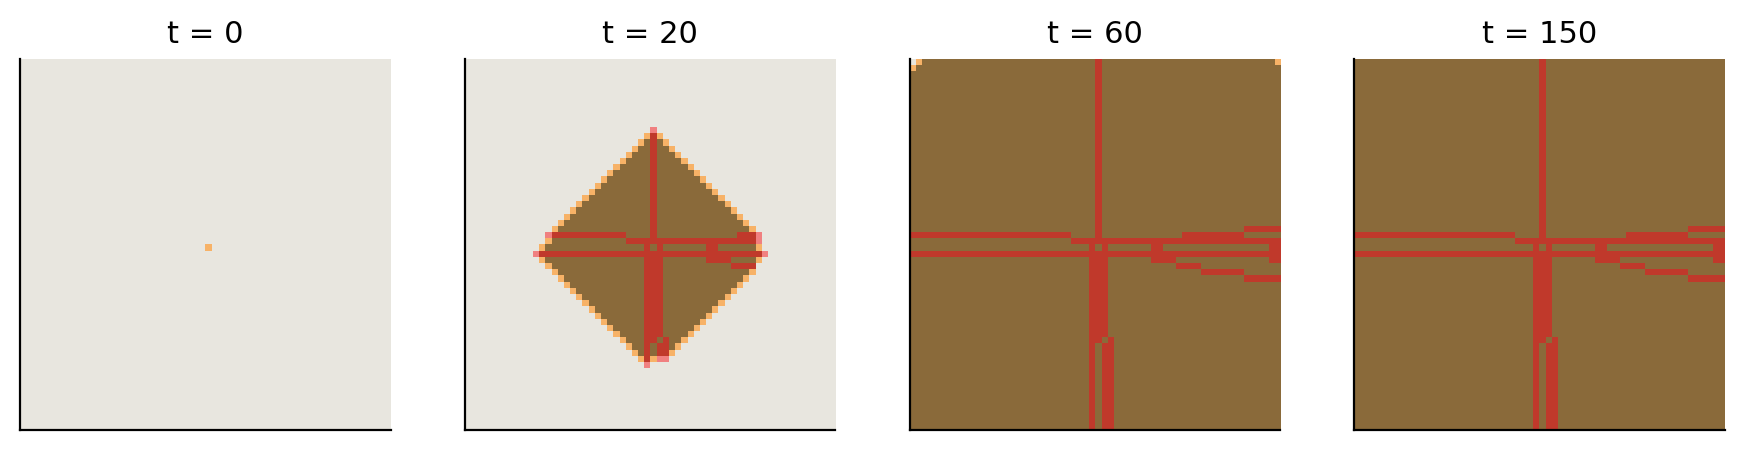
\includegraphics[width=\textwidth]{figures/fig1_cascade.png}
\caption{A cascade at $\alpha = 0.6$, $\theta = 0.80$, from a single seeded
cell, over the stated 150-step horizon. Red cells were removed directly by the
detector; brown cells overloaded after their neighbours had gone. With the
detector disabled at this spare capacity, only the seeded cell is lost.}
\label{fig:cascade}
\end{figure}

\paragraph{Damage is U-shaped, and the collapse is a transition (H1).}
Under a background fault rate and the shared rule, total damage falls from
$2.283$ with the detector effectively disabled to a minimum of $0.142$ at
$\theta = 1.00$, then rises to total loss below $\theta \approx 0.96$
(Figure~\ref{fig:ucurve}a). The arms differ in composition: the permissive arm
is entirely unremediated fault-time, the aggressive arm overload and
false-positive quarantine. The collapse is not gradual---damage
changes by 26\% for a $0.01$ change in threshold, from $0.699$ to $0.947$
between $\theta = 0.94$ and $0.93$---so an operator tightening a threshold to
catch a few more real faults receives little warning. Susceptibility over the
aggressive arm peaks at $\theta = 0.95$, consistent with that step.

\begin{figure}[t]
\centering
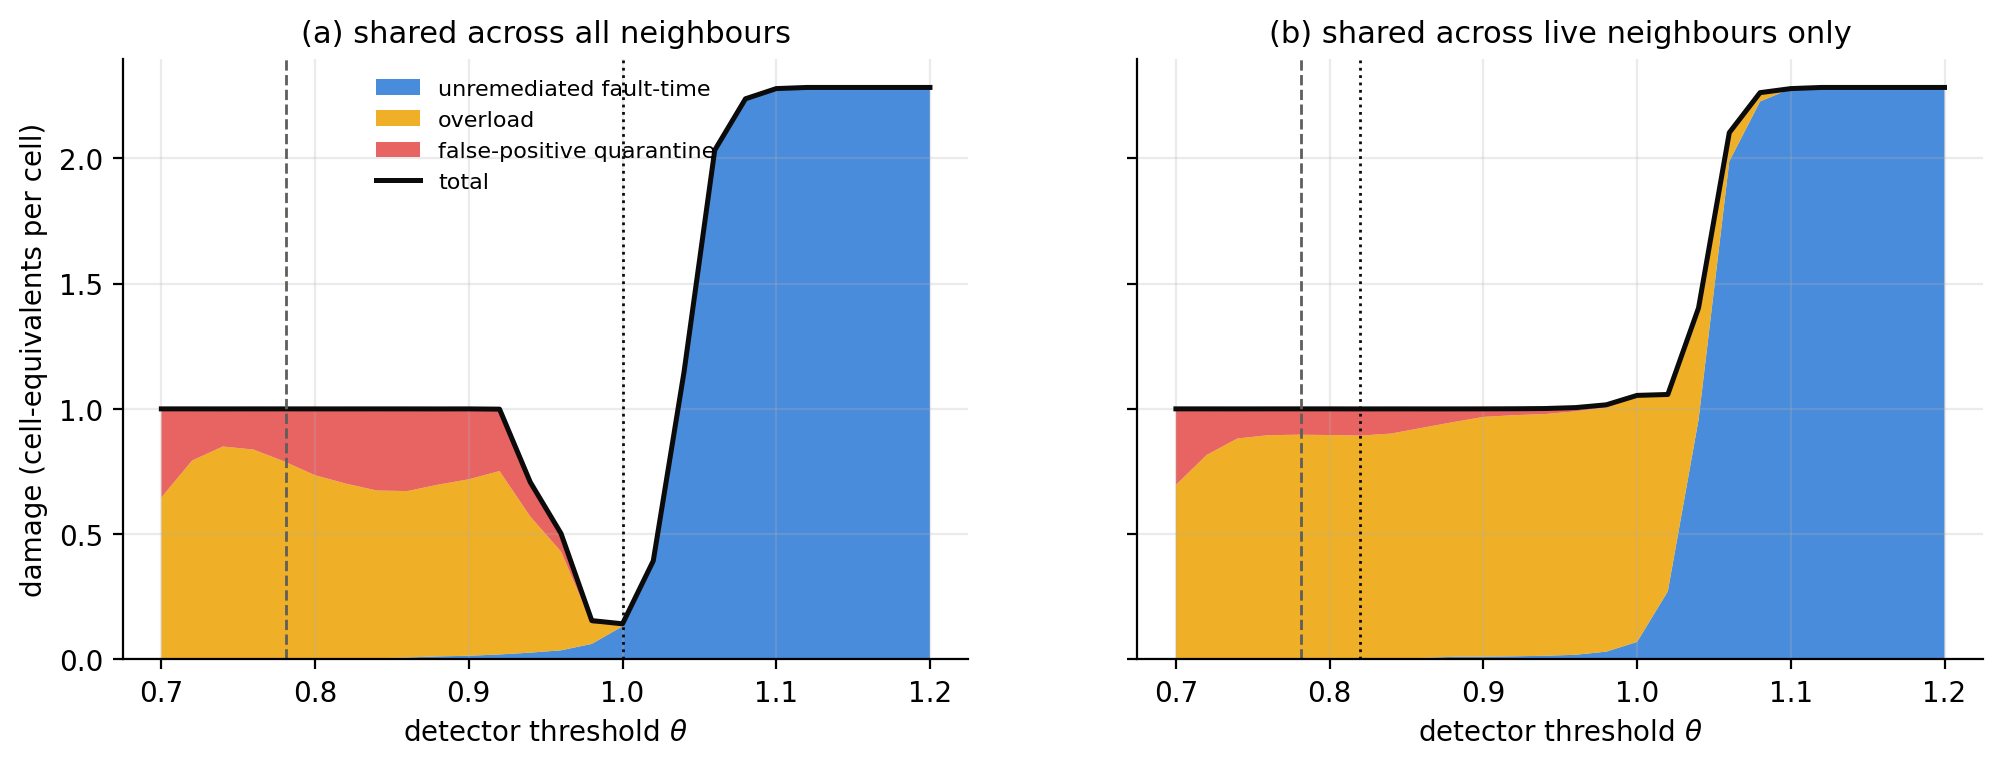
\includegraphics[width=\textwidth]{figures/fig3_ucurve.png}
\caption{Damage decomposed by cause against detector threshold at
$\alpha = 0.6$, under the two redistribution rules. Dotted line: the empirical
optimum. Dashed line: the analytic $\theta_c$. Note that the detector becomes
\emph{less} sensitive to the right. The valley present in (a) is absent in (b).}
\label{fig:ucurve}
\end{figure}

\paragraph{The optimum is a near-constant multiple of the analytic threshold.}
Across $\alpha \in [0.4, 1.0]$ the ratio $\theta^*/\theta_c$ takes the values
$1.19$, $1.28$, $1.30$ and $1.31$, averaging $1.27$, so a safe setting can be
estimated from spare capacity and mean connectivity rather than found by tuning,
though the constant would move with the relative cost of a missed fault.

\paragraph{A separability condition determines whether safety is possible.}
A usable threshold must lie above the reading of a healthy cell that has
absorbed a dead neighbour and below that of a degraded cell: a window of width
$\delta - (1/|N|)/(1+\alpha)$. Measured onsets sit four to six standard
deviations above this floor across four capacity levels:
\begin{equation}
\delta > \frac{1/|N|}{1+\alpha} + z\sigma, \qquad z \approx 4\text{--}6.
\label{eq:sep}
\end{equation}
Automated remediation can be operated safely only if its detector separates
genuine faults from load-induced elevation by several times the telemetry noise;
below that no tuning helps, because the problem is the signal, not the
threshold.

\paragraph{Topology changes the shape of failure, not the safe threshold (H3).}
Re-implementing the automaton with graph neighbourhoods reproduces the lattice
results exactly when given the lattice's own neighbourhood, establishing that
the comparison is controlled. Holding node count and mean degree fixed under the
shared rule, the lattice, small-world and random graphs are strictly
bimodal---0\% of failures are of intermediate size---whereas the scale-free graph
gives 33.3\% intermediate outcomes and never loses the whole platform
(Figure~\ref{fig:topology}a). Since small-world has under half the lattice's
path length but comparable degree spread and behaves like the lattice, the
driver is degree spread rather than distance. The local threshold $\alpha \geq 1/k_j$, set by the degree of the
\emph{failing} cell, holds exactly: across 800 trials no cascade propagated from
a cell of degree $\geq 1/\alpha$, while 57.4\% of those seeded below it did.

\begin{figure}[t]
\centering
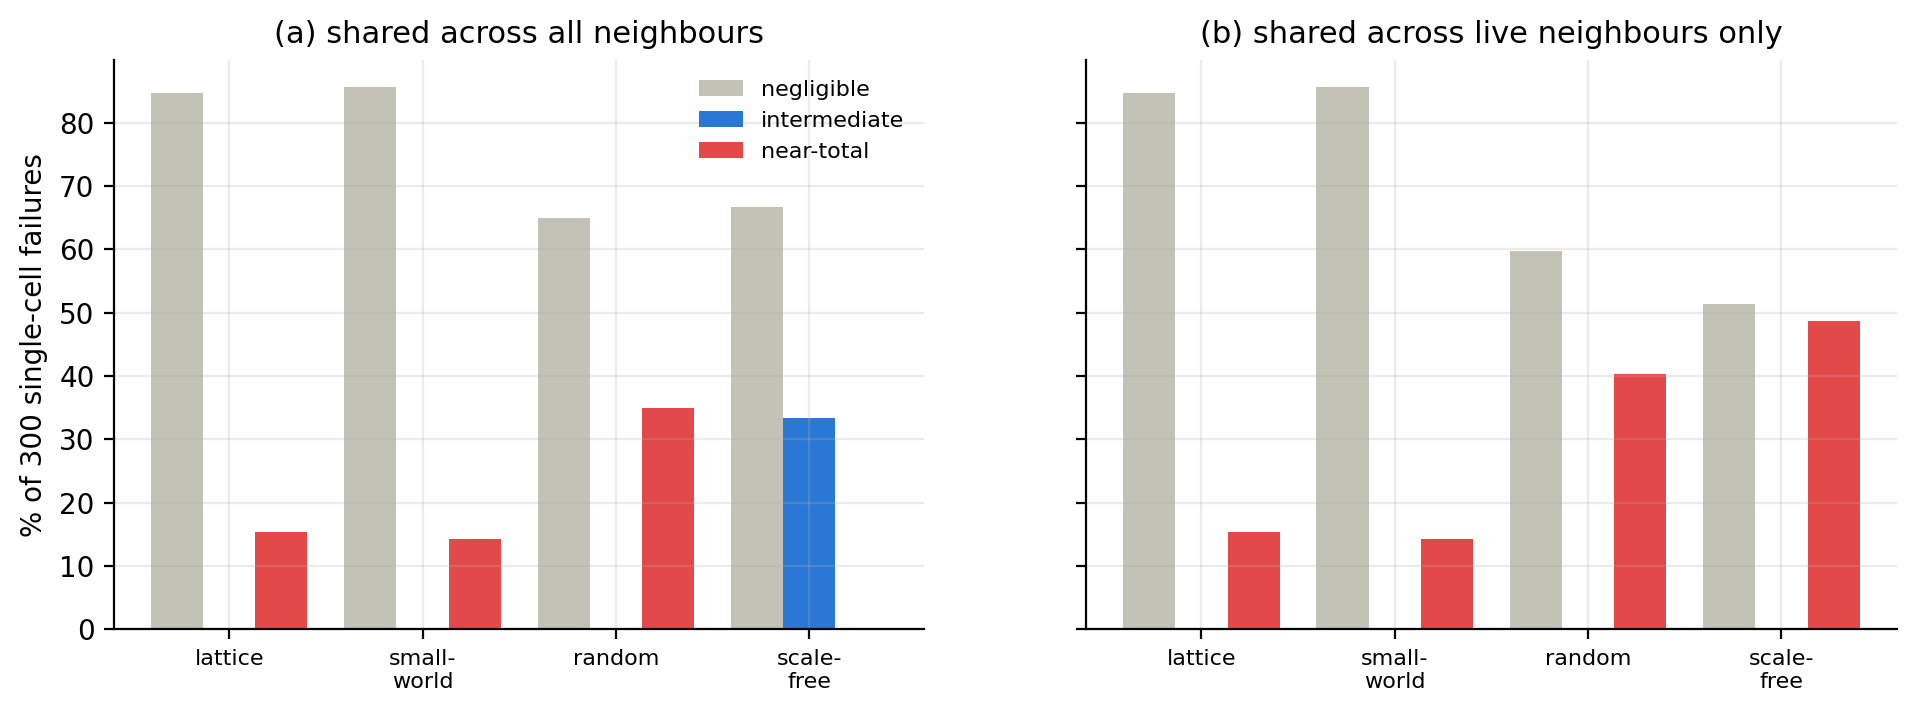
\includegraphics[width=\textwidth]{figures/fig4_topology.png}
\caption{Outcome classification for 300 single-cell failures per topology at
matched $N = 900$ and mean degree 4, under the two redistribution rules. The
intermediate outcomes that distinguish the scale-free graph in (a) are absent
in (b).}
\label{fig:topology}
\end{figure}

\paragraph{Two central results are conditional on the redistribution rule.}
Repeating both experiments under the live-only rule changes them qualitatively,
not merely quantitatively. The U-curve's valley closes: the minimum damage over
the swept range is $1.000$, so every threshold either destroys the platform or
misses the faults (Figure~\ref{fig:ucurve}b). The scale-free graph's
intermediate outcomes fall from 33.3\% to 0\% and near-total losses rise from
0\% to 48.7\% (Figure~\ref{fig:topology}b), so the firebreak behaviour
disappears. Both follow from one cause: concentrating spill on fewer recipients
raises the load signal, narrowing the separability window of
Equation~\ref{eq:sep}. That explanation is testable and holds---on a smaller
lattice where the valley survives, raising $\delta$ from $0.35$ to $0.50$
improves the live-only minimum from $0.715$ to $0.190$. Seeding the five
highest-degree cells still produces no cascade under either rule, so hubs remain
locally safe to lose.

\section{Discussion and conclusions}
\label{sec:disc}

The results support H1 and H2 under the shared rule, and H3 in qualified form:
topology alters the character of failure without appreciably moving the safe
threshold. Whether a safe operating point exists at all depends not only on the
detector but on how a failing instance's traffic is reallocated---a detail of
load-balancer behaviour not normally treated as a safety parameter, and absent
from every cascade model we build on.

The practical reading is uncomfortable. Because the collapse is a transition,
tuning a threshold downward gives little observable degradation until the
platform is lost, so adjusting a parameter until the metrics look wrong gives
limited protection. Because detector
accuracy does not enter Equation~\ref{eq:thetac}, an organisation that responds
to missed faults by improving its model and then tightening its threshold may
move closer to the cliff while believing it has moved away. The more useful
question is therefore whether the detector's signal exceeds load-induced
elevation by a sufficient margin---measurable from production telemetry without
any simulation.

Several limitations bound these conclusions. Capacity is scalar where real
services exhaust resources independently; cells are binary where real services
degrade gracefully; the synchronous schedule omits queueing delay. Removal is
permanent within an episode, so the system can only decay: damage totals are an
upper bound, and the oscillation a delayed recovery would produce is precluded.
Independent detector errors are conservative, since correlated telemetry would
cluster false positives. All results are finite-window observations.

Two extensions follow: quarantine recovery would add a delayed negative feedback
opposing the positive feedback studied here, plausibly converting collapse into
oscillation; and calibrating $\delta$ and $\sigma$ against production telemetry
would turn Equation~\ref{eq:sep} into an operational test.

We conclude that automated remediation is best understood not as a control
system acting on a platform but as a second failure process running on it, one
competing with the faults it is meant to remove and capable of dominating them.
The design question is accordingly not how accurately faults can be detected,
but how much of the platform an automated response may remove---and where that
traffic is then sent---before the removal itself becomes the outage.



\appendix
\section{Protocol verification}
\label{app:protocol}

Each of the four protocol choices in Section~5 replaced an earlier treatment
that an audit of the implementation found unsound. The five corrections are
documented individually, with before-and-after validation, in
\texttt{docs/Correction Report.md}; this appendix records the evidence that each
is now correct.

\paragraph{Observation horizon.}
Under the earlier rule a trial stopped at the first timestep in which no cell
changed state. With noise or faults still arriving this is not a fixed point.
The $60\times60$ example at $\alpha = 0.6$, $\theta = 0.80$, $\sigma = 0.02$ and
seed 3 stopped after two steps having lost one cell; over the stated 150-step
horizon it loses all 3600. The implementation now refuses to run a convergence
loop when stochastic input is present, raising an error that directs the caller
to the fixed-horizon routine, so the earlier mistake cannot recur silently.

\paragraph{Paired random inputs.}
Because a disabled detector never calls the telemetry function, it never drew
noise and so advanced the shared generator differently from an enabled
detector, giving the two a different fault sequence at the same seed. Comparing
a disabled detector against a very high threshold on a $6\times6$ lattice at
seed 7: under the shared stream the two state sequences agree at step 1 and
diverge from step 2 onward; under split streams they agree at every step.

\paragraph{Load accounting.}
Load addressed to a cell that had already been removed previously left the
system unrecorded. On a $7\times7$ lattice with a second failure adjacent to an
existing corpse, the shared rule now holds $47.70$ units live with $1.30$
recorded as dropped, against an initial $49$; the live-only rule holds all $49$
with none dropped. Both account for the initial total.

\paragraph{Reproducibility.}
Degree-ordered demonstration selections previously depended on an unspecified
tie-break among equal-degree cells and could differ between environments. Ties
now break by ascending cell index. The validated environment --- CPython
3.12.14, NumPy 2.5.3, NetworkX 3.6.1, Matplotlib 3.11.2 --- is pinned in
\texttt{requirements-repro.txt}.

\section*{Code, data and runnable simulations}
\begin{sloppypar}
\noindent\url{https://github.com/Aniket-k-159/AutoImmune-Cloud}. Three
notebooks reproduce the results in order: \path{01_cellular_automaton.ipynb}
(gates, U-curve), \path{02_topology_comparison.ipynb} (H3) and
\path{03_robustness.ipynb} (sensitivity, separability).
\path{experiments/report_numbers.py} regenerates every number quoted here;
\path{experiments/validate_lattice.py} re-checks every analytic gate; the five
implementation corrections are documented with before-and-after validation in
\path{docs/corrections.md}.
\end{sloppypar}

\begin{thebibliography}{9}
\small
\bibitem[Albert et al.(2000)]{albert2000} Albert, R., Jeong, H., \& Barab\'{a}si, A.-L. (2000).
Error and attack tolerance of complex networks. \emph{Nature}, 406, 378--382.
\bibitem[Bak et al.(1987)]{bak1987} Bak, P., Tang, C., \& Wiesenfeld, K. (1987). Self-organized
criticality: an explanation of 1/f noise. \emph{Physical Review Letters},
59(4), 381--384.
\bibitem[Clauset et al.(2009)]{clauset2009} Clauset, A., Shalizi, C. R., \& Newman, M. E. J. (2009).
Power-law distributions in empirical data. \emph{SIAM Review}, 51(4), 661--703.
\bibitem[Downey(2018)]{downey2018} Downey, A. B. (2018). \emph{Think Complexity: Complexity
Science and Computational Modeling} (2nd ed.). O'Reilly Media.
\bibitem[Drossel \& Schwabl(1992)]{drossel1992} Drossel, B., \& Schwabl, F. (1992). Self-organized
critical forest-fire model. \emph{Physical Review Letters}, 69(11), 1629--1632.
\bibitem[Motter \& Lai(2002)]{motter2002} Motter, A. E., \& Lai, Y.-C. (2002). Cascade-based attacks
on complex networks. \emph{Physical Review E}, 66(6), 065102.
\end{thebibliography}

\end{document}
